%-------------------------------------------------------------
\documentclass{beamer}
\usepackage[utf8]{inputenc}
\usepackage{hyperref}
\usepackage[T1]{fontenc}
\usepackage{tikz}

\usepackage{latexsym,xcolor,multicol,booktabs,calligra}
\usepackage{amsmath,amssymb,BOONDOX-cal,bm}	
\usepackage{graphicx,pstricks,stackengine}      


\author{Michael Curry}
\title{Data Augmentation for CNN construction using Pixel Blending Modes}
\institute{SUNY New Paltz} 


\usepackage{Wue}

\def\cmd#1{\texttt{\color{red}\footnotesize $\backslash$#1}}
\def\env#1{\texttt{\color{blue}\footnotesize #1}}

\newtheorem{thm}{Theorem}[theorem]


%—-------------------------------------------------------------

\begin{document}
	\begin{frame}
    \titlepage
    \end{frame}

	
	\begin{frame}
		\tableofcontents[sectionstyle=show,subsectionstyle=show/shaded/hide,subsubsectionstyle=show/shaded/hide]
	\end{frame}
		
	
	%—------------------------------------------------------
	\section{HDR Images}
	    %\subsection{}
		    \begin{frame}
			    \begin{itemize} 
			    \item Test
			    \end{itemize}
		    \end{frame}
	
	%-------------------------------------------------------	
	\section{LDR Images}
	    %\subsection{}
		    \begin{frame}
			    \begin{enumerate}
			    \item Test
			    \end{enumerate}	
		    \end{frame}
	
	%-----------------------------------------------------
	\section{HDR image construction from LDR}
	    %\subsection{}
	
	\begin{frame}
		\begin{itemize}
		\item 1
		\end{itemize}
	\end{frame}
		
	\begin{frame}
		\begin{enumerate}
		\item 2
		\end{enumerate}
	\end{frame}
	
	\subsection{Test}
	
	\begin{frame}
    	\begin{itemize}
    	\item Test
    	\end{itemize}
        \begin{table}[h]
    		\centering
    		\begin{tabular}{c|c}
    			Microsoft Word & \LaTeX{} \\
    			\hline
    			Test & 0\\
    			Test & 1\\
    			Test & 2\\
    		\end{tabular}
    	\end{table}
    \end{frame}
	
    \begin{frame}
	    \begin{exampleblock}{Test} 
    		\begin{equation*}
    		f(x)=ax+b 
    		\label{eq1}
    		\end{equation*}
    	\end{exampleblock}
	
    	\begin{exampleblock}{Test\footnote{\tiny Test123}}
    		\begin{align}
    		    \vec{x}
    		    \begin{cases}
    			1 & 2\\
    			0 & 3\\
    		    \end{cases}
    	    	\label{eq2}
    		\end{align}
    	\end{exampleblock}
    \end{frame}
	
	\begin{frame}
		\begin{exampleblock}{Test}
		
			\begin{multline}
			A=1+\\
			2+\\
			3+\\
			4+\\
			5+\\
			=15
			\end{multline}
		\end{exampleblock}
	\end{frame}
	
	\begin{frame}{Test}
 
		\begin{columns}[T]
			\begin{column}<0->{.5\textwidth}
				\begin{figure}[thpb]
					\centering
					\resizebox{1\linewidth}{!}{
						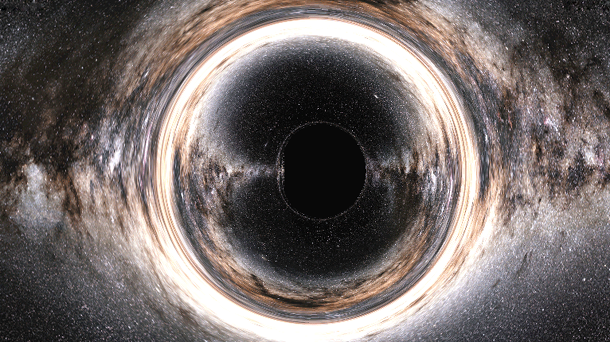
\includegraphics{Black-7c99d21dddbb1ba2.png}
					}
					%	\includegraphics[scale=1.0]{figurefile}
					\caption{Test}
					\label{fig:1}
				\end{figure}
			\end{column}%
			\hfill%
			\begin{column}<0->{.5\textwidth}
				\begin{itemize}
					\item<1-> Test
					\begin{itemize}
						\item<1-> Test 2
					\end{itemize}
					\item<2-> Test
					\begin{itemize}
						\item<2-> Test 3
					\end{itemize}
				\end{itemize}
			\end{column}
		\end{columns}
	\end{frame}

	\begin{frame}[fragile]{\LaTeX{} Test}
		\begin{exampleblock}{Test}
			\centering
			\footnotesize
			\begin{tabular}{llll}
				1&2&3&4
			\end{tabular}
		\end{exampleblock}
		\begin{exampleblock}{Test}
			\centering
			\footnotesize
			\begin{tabular}{lll}
				1&2&3
			\end{tabular}
		\end{exampleblock}
	\end{frame}
	
	%-------------------------------------------------
	\section{Chapter 4}	
	
	\begin{frame}<1->
		 \begin{thm}
	        contents...
	        \label{thm-1}
		 \end{thm}
		\begin{block}{Test}<2->
            This is a theorem.
            \begin{equation}
                a^2 + b^2 = c^2
            	\notag	
            	\label{equ-3}
            	\end{equation}
        \end{block}
    	
		\begin{proof}<3->
            \textit{Trivial.} 
        \end{proof}
		            
        \begin{corollary}<4->
            This is a corollay.
            \begin{equation}
                c^2 = b^2 + a^2
                \label{equ-4}
            \end{equation}
        \end{corollary}
	\end{frame}
	
	\begin{frame}{Test}
		\begin{itemize}
			\item Test 1
			\begin{itemize}
				\item Test
				\item Test
				\item Test 
			\end{itemize}
			\item Test
			\begin{itemize}
				\item 1
				\item 2
			\end{itemize}
		\item 3
		\end{itemize}
		
	\end{frame}

	%----------------------------------------------
%	\section{References}
%		
%		\begin{frame}[allowframebreaks]
%			\bibliographystyle{unsrt}
%			\bibliography{Bibliography.bib}	
%		\end{frame}
%%
	%-------------------------------------------
%	\begin{frame}
%		\begin{center}
%			{\Huge \emph {\textrm{Thank  ~you!}}}
%		\end{center}
%	\end{frame}

\end{document}